\documentclass[10pt]{beamer}
\usetheme[
%%% options passed to the outer theme
%    hidetitle,           % hide the (short) title in the sidebar
%    hideauthor,          % hide the (short) author in the sidebar
%    hideinstitute,       % hide the (short) institute in the bottom of the sidebar
%    shownavsym,          % show the navigation symbols
%    width=2cm,           % width of the sidebar (default is 2 cm)
%    hideothersubsections,% hide all subsections but the subsections in the current section
%    hideallsubsections,  % hide all subsections
%    left                % right of left position of sidebar (default is right)
 ]{Aalborg}
  
% If you want to change the colors of the various elements in the theme, edit and uncomment the following lines
% Change the bar and sidebar colors:
%\setbeamercolor{Aalborg}{fg=red!20,bg=red}
%\setbeamercolor{sidebar}{bg=red!20}
% Change the color of the structural elements:
%\setbeamercolor{structure}{fg=red}
% Change the frame title text color:
%\setbeamercolor{frametitle}{fg=blue}
% Change the normal text color background:
%\setbeamercolor{normal text}{bg=gray!10}
% ... and you can of course change a lot more - see the beamer user manual.

\usepackage[utf8]{inputenc}
\usepackage[english]{babel}
\usepackage[T1]{fontenc}
\usepackage{amsmath}
\usepackage{graphicx}
\usepackage{multimedia}

% Or whatever. Note that the encoding and the font should match. If T1
% does not look nice, try deleting the line with the fontenc.
\usepackage{helvet}

\newcommand{\Vector}[1]{\mathbf{#1}}
% colored hyperlinks
\newcommand{\chref}[2]{%
  \href{#1}{{\usebeamercolor[bg]{Aalborg}#2}}%
}
\newcommand{\del}{\partial}
\title[Symmetry Reduced Exact Coherent Structures in Plane Couette Flow]% optional, use only with long paper titles
{Symmetry Reduced Exact Coherent Structures in Plane Couette Flow}

\subtitle{}  % could also be a conference name

\date{\today}

\author[] % optional, use only with lots of authors
{
  Varchas Gopalaswamy
% \href{mailto:jkn@es.aau.dk}{{\tt jkn@es.aau.dk}}
}
% - Give the names in the same order as they appear in the paper.
% - Use the \inst{?} command only if the authors have different
%   affiliation. See the beamer manual for an example

\institute[
%  {\includegraphics[scale=0.2]{aau_segl}}\\ %insert a company, department or university logo
  Dept.\ of Physics\\
  Reed College
] % optional - is placed in the bottom of the sidebar on every slide
{% is placed on the bottom of the title page
  Department of Physics\\
  Reed College
  
  %there must be an empty line above this line - otherwise some unwanted space is added between the university and the country (I do not know why;( )
}

% specify the logo in the top right/left of the slide
\pgfdeclareimage[height=1cm]{mainlogo}{AAUgraphics/reed_logo} % placed in the upper left/right corner
\logo{\pgfuseimage{mainlogo}}

% specify a logo on the titlepage (you can specify additional logos an include them in 
% institute command below
\pgfdeclareimage[height=1.5cm]{titlepagelogo}{AAUgraphics/reed_logo} % placed on the title page
%\pgfdeclareimage[height=1.5cm]{titlepagelogo2}{AAUgraphics/aau_logo_new} % placed on the title page
\titlegraphic{% is placed on the bottom of the title page
  \pgfuseimage{titlepagelogo}
%  \hspace{1cm}\pgfuseimage{titlepagelogo2}
}

\begin{document}
% the titlepage
{\aauwavesbg
\begin{frame}[plain,noframenumbering] % the plain option removes the sidebar and header from the title page
  \titlepage
\end{frame}}
\begin{frame}
\movie[autostart,loop]{\includegraphics{Images/PhaseSpaceTraj}}{Videos/P85.avi}
\end{frame}
\section{The Problem}
\begin{frame}{Turbulence}{}
\begin{block}{What is it, and why do we care?}
  \begin{itemize}
    \item<1->Turbulence is an irregular, chaotic, and dissipative flow phenomenon, with a vast number of (coupled) length scales. 
  \end{itemize}
\begin{tabular}{cc}
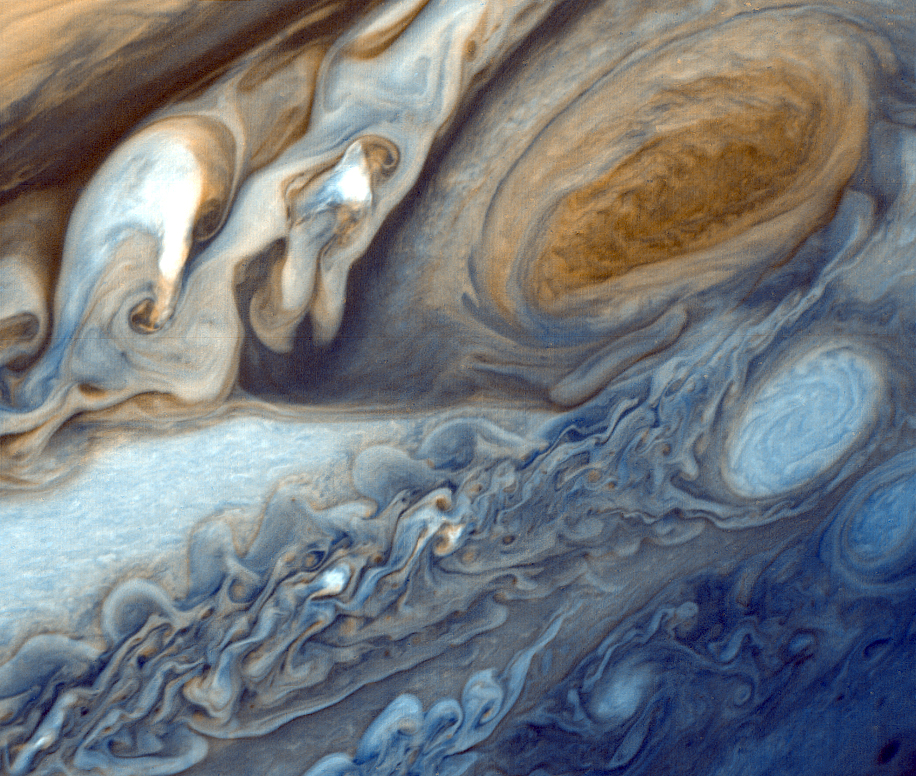
\includegraphics[scale=0.1]{Images/jupiter-v1} & 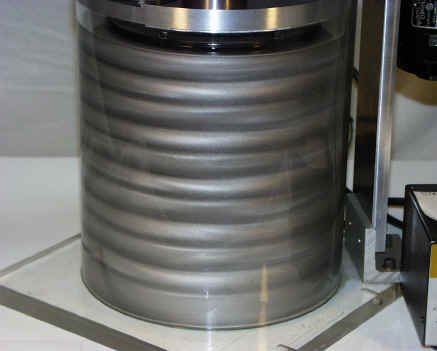
\includegraphics[scale=0.4]{Images/TaylorCouette_Banded}
\end{tabular}
\begin{itemize}
\item<1-> Shows up in many important systems - atmospheric and geophysical flows, turbine exhaust, stellar flows...
\item<2-> Direct numerical simulation (DNS) is very time consuming - need a simpler model! 
\end{itemize}
\end{block}
\end{frame}

\subsection{Transitions to Turbulence}
\begin{frame}{Transitions to Turbulence}
\begin{itemize}
\item<1-> Of particular inteerest are transitions to turbulence from smooth (laminar) flow
\end{itemize}
\begin{figure}
\begin{tabular}{cc}
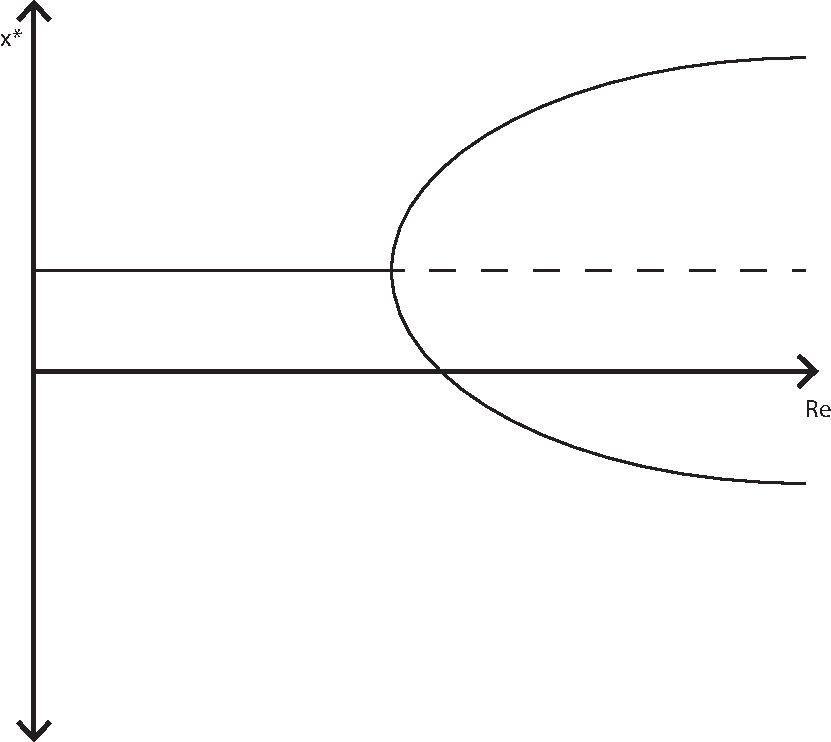
\includegraphics[scale=0.3]{Images/supercriticalTrans} & 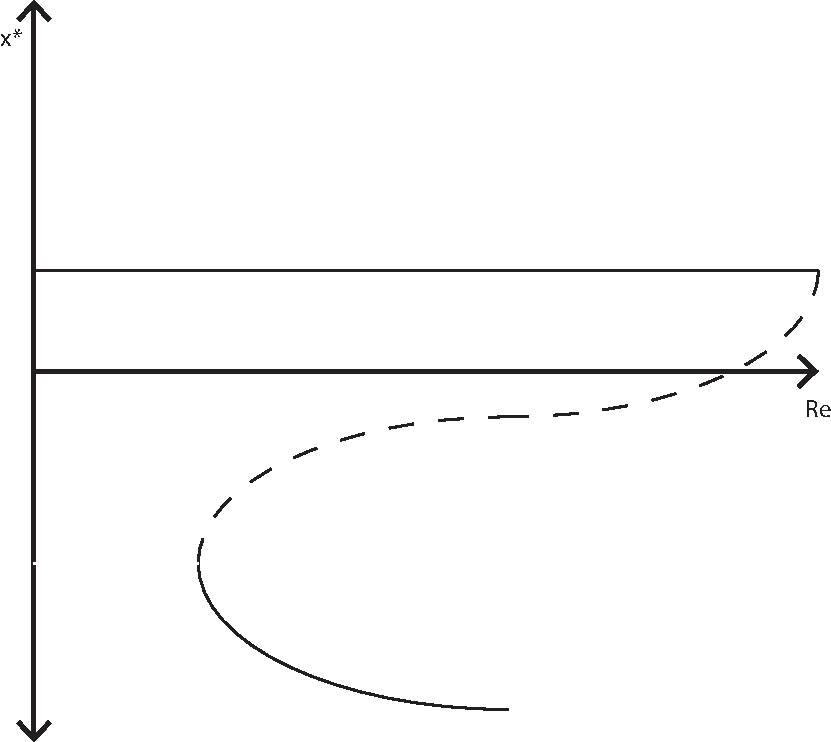
\includegraphics[scale=0.3]{Images/subcriticalTrans}\\
{\small Supercritical Transition} & {\small Subcritical Transition}
\end{tabular}
\end{figure}
\end{frame}
\begin{frame}{Transitions to Turbulence} 
\begin{itemize}
\item<1-> Supercritical transitions are well described by linear stability analysis (inner-cylinder rotation in Taylor Couette flow)...
\item<2-> Subcritical transitions are sudden and unpredictable (pipe flow, plane Couette flow)
\end{itemize}
\end{frame}

\section{The System}
\subsection{Navier-Stokes}
\begin{frame}{The System}{Navier-Stokes}
The Navier-Stokes equation is the linear momentum conservation statement for Newtonian, incompressible fluids:
\begin{equation*}
 \left(\frac{\partial \mathbf{v}}{\partial t} + \mathbf{v} \cdot \nabla \mathbf{v}\right) = -\nabla p + \dfrac{1}{Re} \nabla^2 \mathbf{v},
\end{equation*}
with the appropriate boundary conditions.
\end{frame}
\subsection{Bulk Flow}
\begin{frame}{The System}{Base Flow}
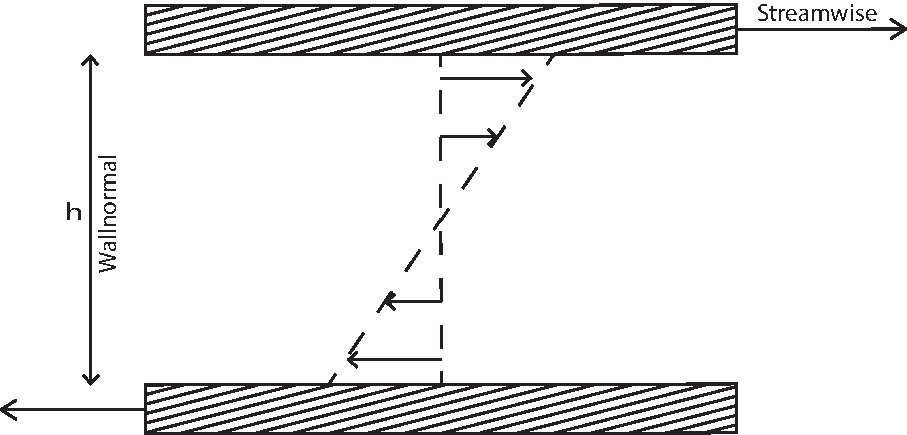
\includegraphics[scale=0.6]{Data/planeCouette}
\end{frame}
\begin{frame}
{The System}{Plane Couette}
If the Reynolds number is not small, the damping term is about the same size as the rest of the terms, and we have to solve the full Navier-Stokes equations (for Couette flow) 
\begin{equation*}
 \left(\frac{\partial \mathbf{v}}{\partial t} + \mathbf{v} \cdot \nabla \mathbf{v}\right) =\dfrac{1}{Re} \nabla^2 \mathbf{v},
\end{equation*}
\end{frame}

%%%%%%%%%%%%%%%%

\subsection{Statistical Methods}
% the license
\begin{frame}{Turbulence}{Statistical Methods}
  \begin{itemize}
    \item<1-> Mean field approaches, such as the Reynolds Averaged Navier Stokes have had a great deal of success
    \item<2-> RANS works by time averaging out the turbulent perturbations to some mean flow, resulting in a new equation of motion for the mean flow...
    \item<3-> ... but dynamical properties of turbulence are lost in the time-averaging process 
  \end{itemize}
\end{frame}
%%%%%%%%%%%%%%%%

\subsection{Exact Coherent Structures} 
\begin{frame}{Turbulence}{Exact Coherent Structures}
\begin{itemize}
	\item<1-> Instead of time averaging the perturbation away, try to analyze its dynamics
	\item<2-> Imagine the perturbation as living in some infinite dimensional space of all possible velocity fields (the `state space') 
\end{itemize}
\end{frame} 
\begin{frame}{Laminar Basin of Attraction}

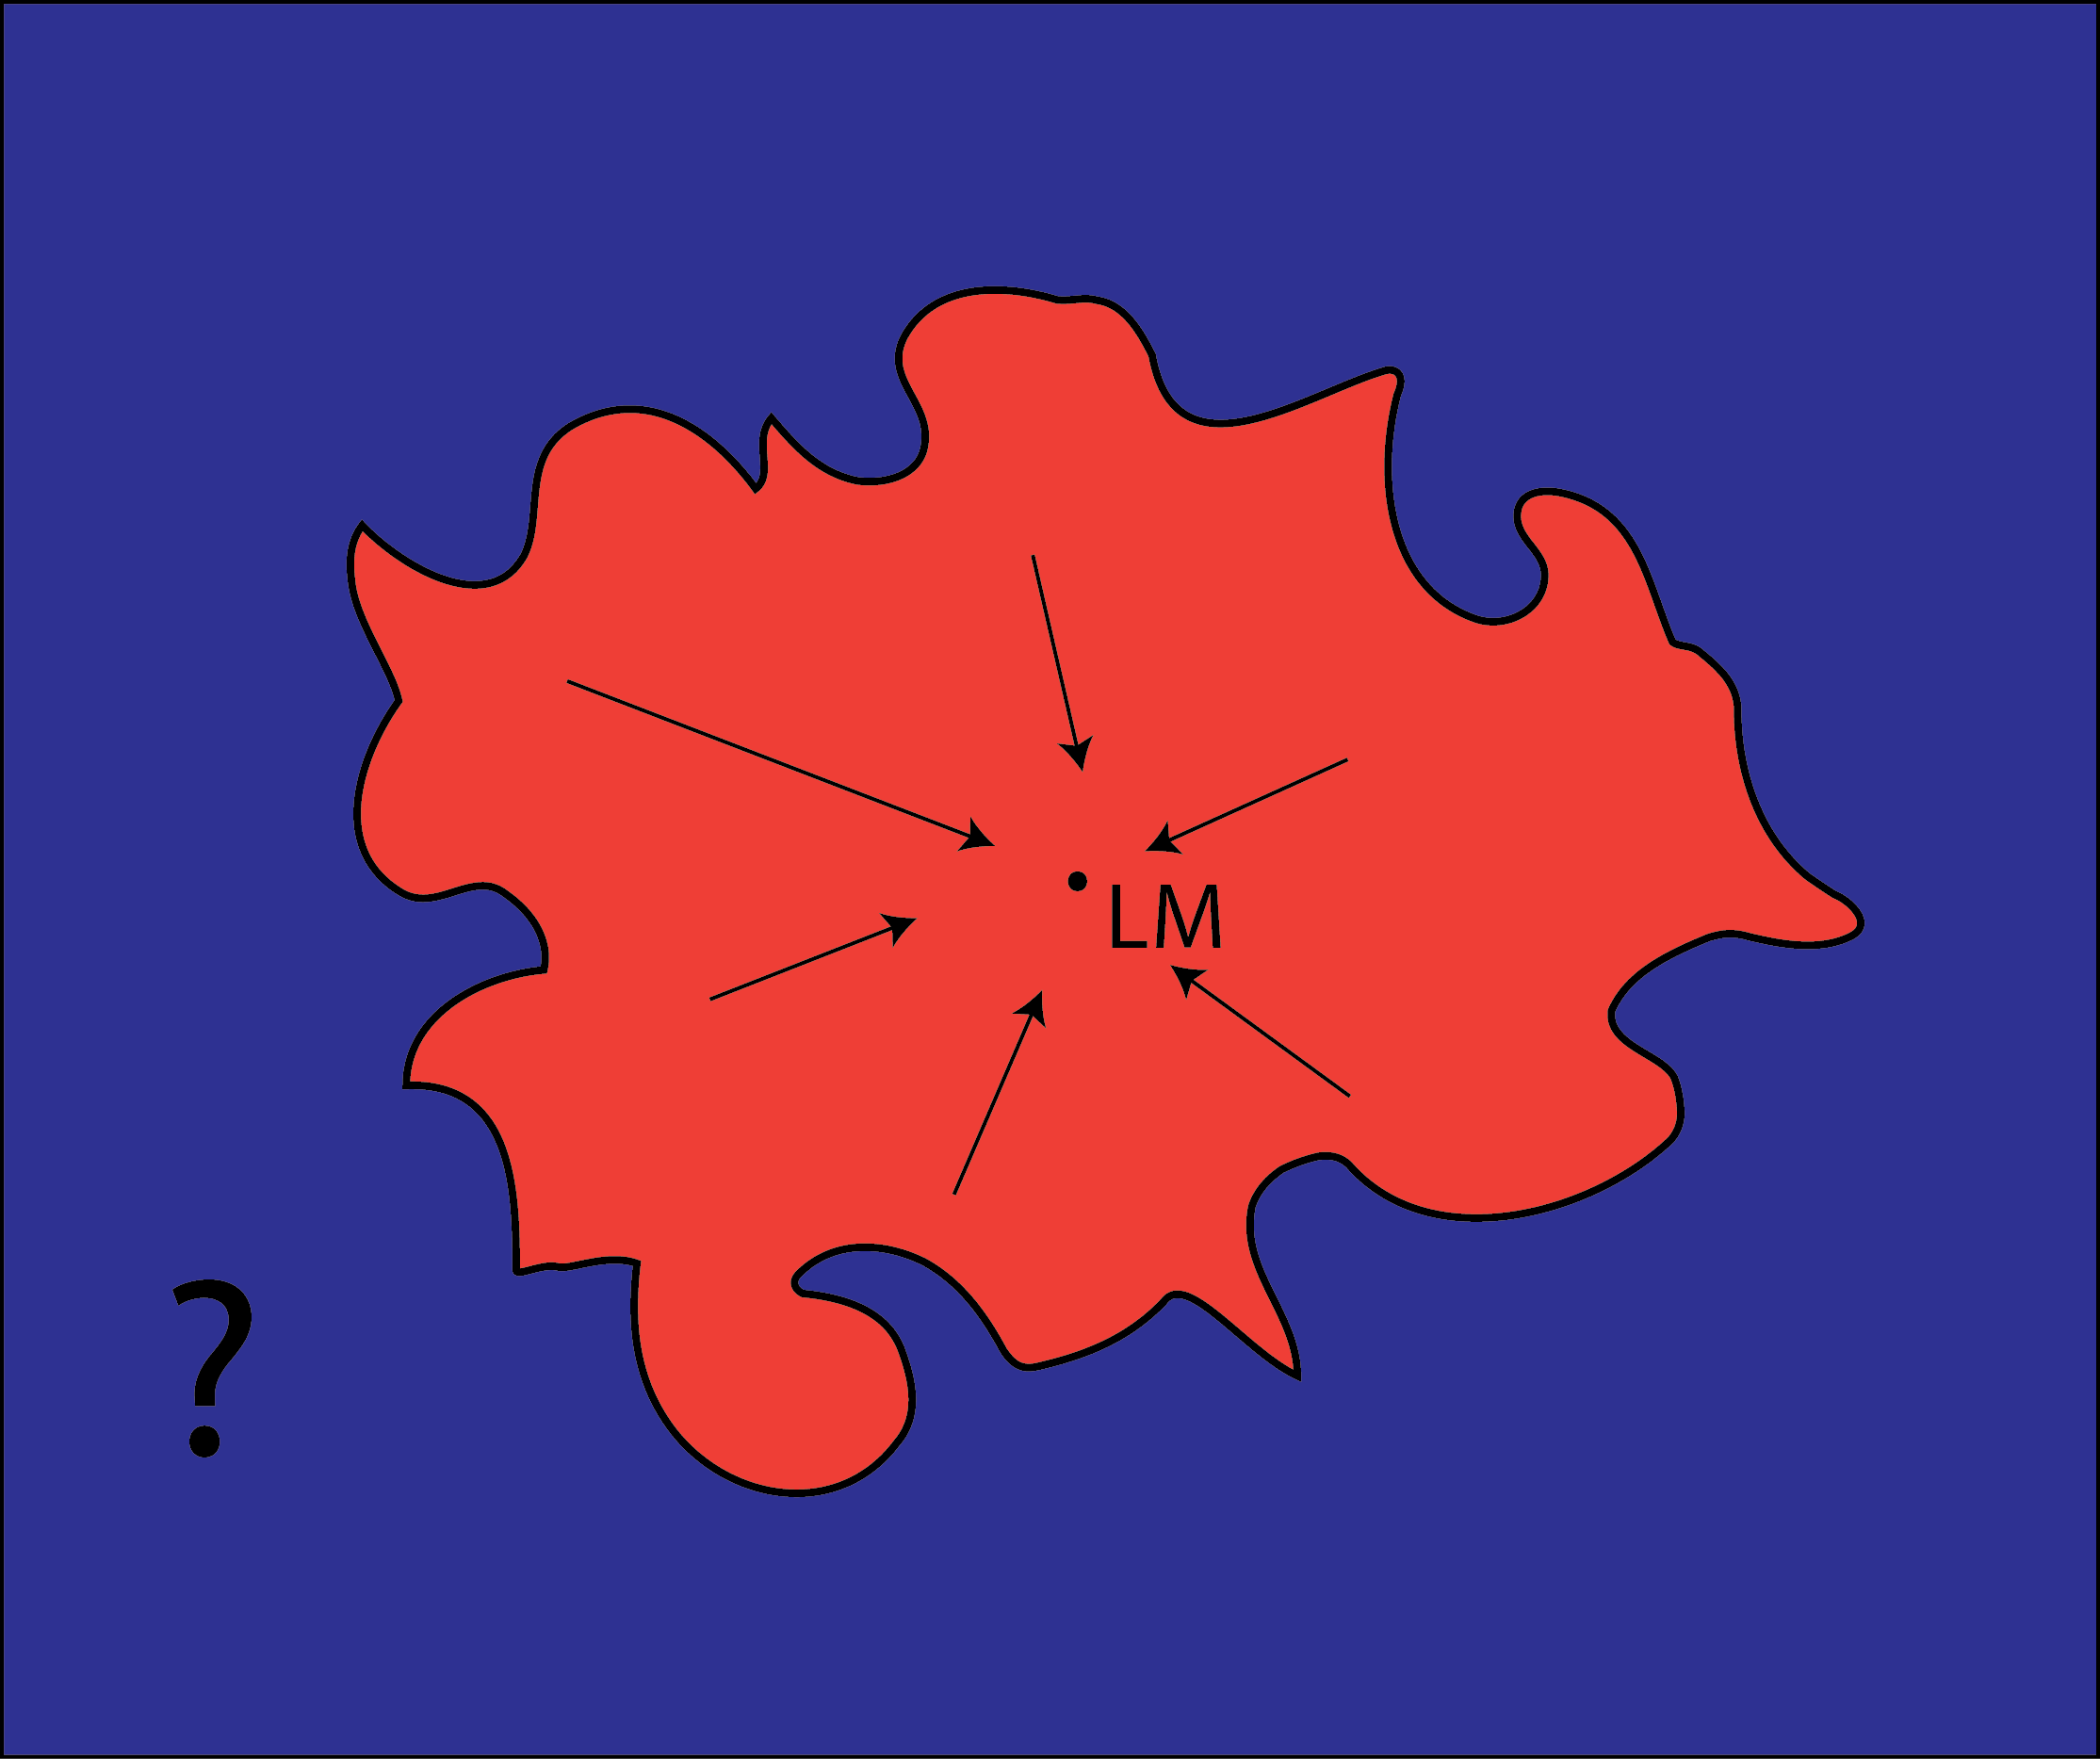
\includegraphics[scale=0.47]{Images/basinOfAttraction.png}
\end{frame}
\begin{frame}{Turbulence}{Equilibria}

\centerline{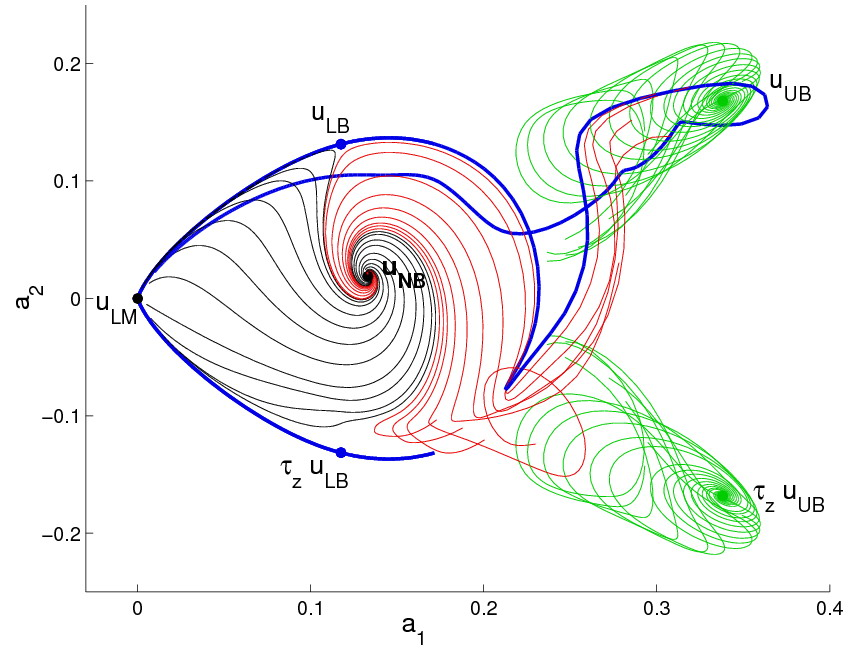
\includegraphics[scale=0.3]{Data/stateSpace}}
\hspace{8\baselineskip} {\footnotesize Halcrow et. al (2008) }

\end{frame} 

\section{Symmetry}

\begin{frame}{Symmetry}
\begin{itemize}
\item<1-> The full Navier-Stokes equations are invariant ($f_T(\sigma\Vector{u}) = \sigma f_T(\Vector{u})$) under any spatial rotation and translation
\item<2-> Boundary conditions of plane Couette flow reduce the number of invariant symmetries to the group generated by the following transformations:
\begin{itemize}
\item<3-> $\sigma_{xy} \rightarrow$ Rotation by $\pi$ about the $z$ axis
\item<4-> $\sigma_{z} \rightarrow $ Mirroring across the $z$ axis
\item<5-> $\tau(l_x,l_z) \rightarrow $ Translation by $(l_x,l_z)$ in the $xz$ plane
\end{itemize}
\end{itemize}
\end{frame}

\begin{frame}{Symmetry}{Relevance to Turbulence}
\begin{itemize}
\item<1-> Integration and root finding in a symmetric subspace are faster - fewer computations required
\item<2-> Coherent structures can also exist in  different inertial reference frames $\rightarrow$ travelling waves
\item<3-> Symmetries can restrict the allowed directions of these travelling waves (Viswanath, 2007). 
\item<4-> Symmetric fields are also not necessarily representative of turbulence

\end{itemize}
\end{frame}
\begin{frame}{Symmetric and Asymmetric Fields}
\begin{figure}
\begin{tabular}{cc}
\includegraphics[scale=0.4]{Data/randomfield.jpg} & 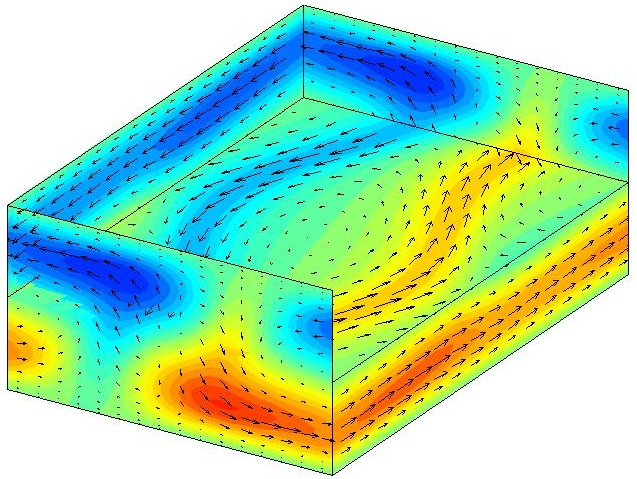
\includegraphics[scale=0.25]{Data/p85p47NoBase}\\
{\footnotesize A random, asymmetric field} & {\footnotesize A highly symmetric periodic orbit}
\end{tabular}
\end{figure}
\end{frame}
%%%%%%%%%%%%%%%%
\section{The Simulation}
\begin{frame}{The Simulation}
\begin{itemize}
\item<1-> I use Channelflow, a simulation library developed at UNH (Gibson, 2014) to analyze plane Couette flows.  
\item<2-> In addition to Navier-Stokes integration, Channelflow can also find coherent structures (with a good initial guess)
\end{itemize}
\end{frame}
\begin{frame}{The Simulation}{Generating a good guess}
\begin{itemize}
\item<1-> How do we hunt through the immense phase space? (> 60,000 dimensions)
\item<2-> Start from a random initial condition
\item<3-> Integrate flow forward in time
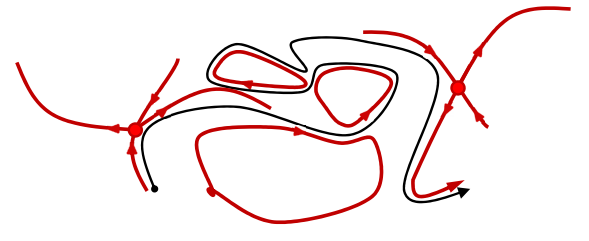
\includegraphics[scale=0.5]{Images/phaseSpaceTraj}
\hspace{10cm}{\footnotesize Borrero (2014)} 
\item<4-> Look at recurrence graphs
\end{itemize}
\end{frame}
\subsection{Recurrence Graphs}
\begin{frame}{The Simulation}{Recurrence Graphs}
\begin{itemize}
\item<1-> Can compare the flow at time $t$ to time $t+T$ by calculating $d(\Vector{u}(t),\Vector{u}(t+T))$
\item<2-> Use the physically motivated energy norm
\end{itemize}
\pause
\begin{equation*}
|\Vector{u}|^2 = \frac{1}{V}\int_V{\Vector{u}\cdot\Vector{u}}{dV},
\end{equation*}
\begin{itemize}
\item<3-> Minima of these plots should indicate the presence of a periodic orbit
\end{itemize}
\end{frame}
\begin{frame}{The Work}{Recurrence Plots}
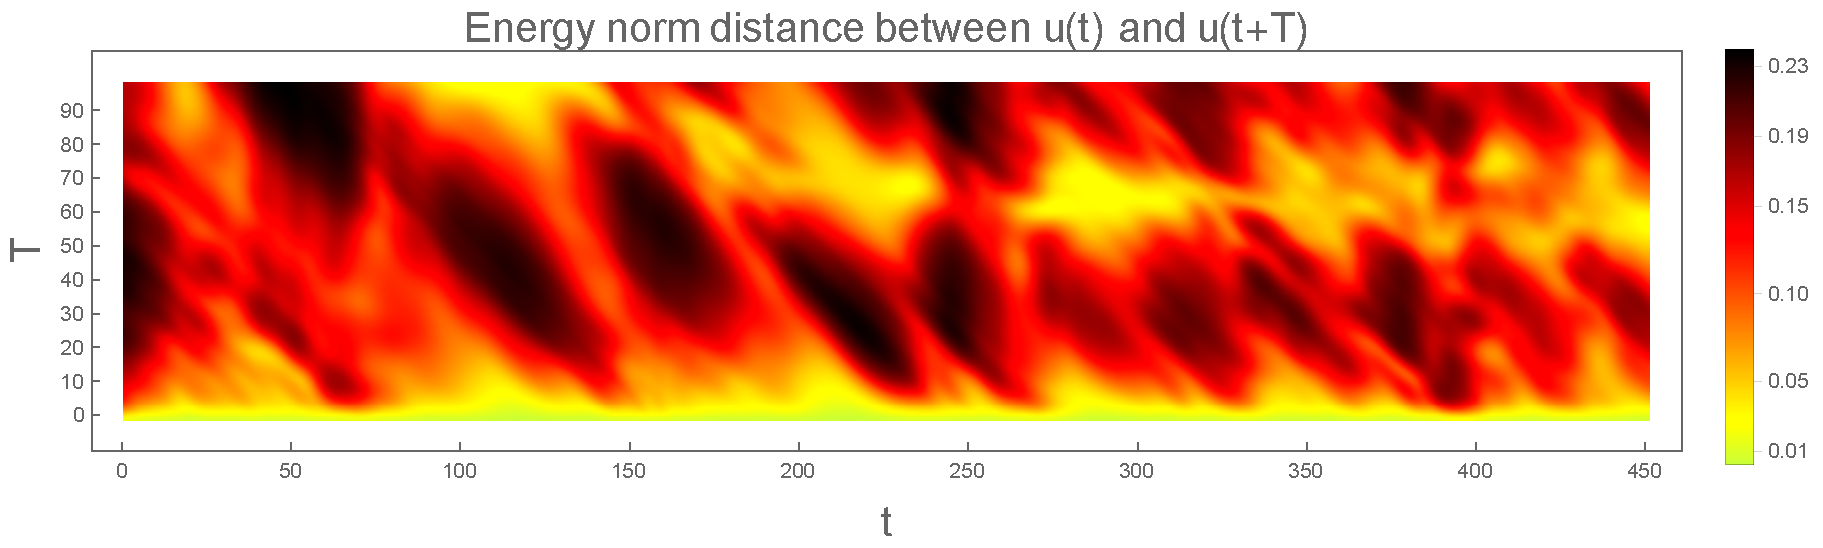
\includegraphics[scale = 0.3]{Data/RecPlot}
\end{frame}
\subsection{Root Finding}
\begin{frame}{The Simulation}{Root Finding}
\begin{itemize}
\item<1-> Once a promising candidate is found, it can be passed on to the root finder, to solve 
\begin{equation*}
\Vector{u} - \sigma f_T(\Vector{u}) = 0,
\end{equation*}
\item<2-> where $\sigma$ encodes the travelling wave velocity.
\item<3-> The root finder uses the Newton method, with the step in 60,000 dimensions calculated using the generalized minimum residual method.  
\end{itemize}
\end{frame}
\section{Current Results}
\begin{frame}{P85.47}
This orbit has period $T = 85.47$, and has symmetries generated by $\{e,\sigma_{xy},\sigma_{z}\tau_{xz}\} $
\vbox{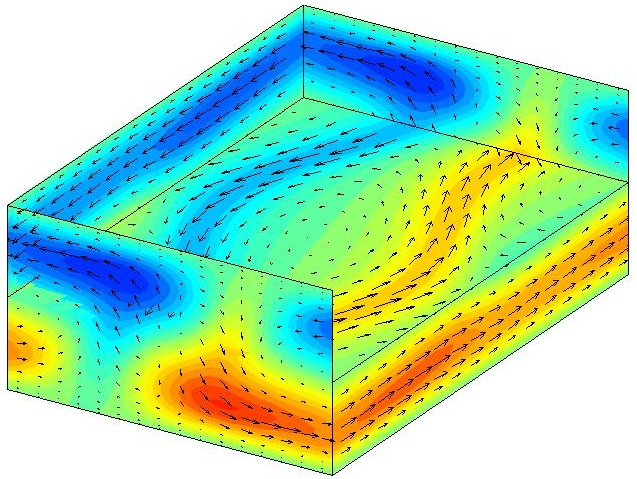
\includegraphics[scale=0.45]{Data/p85p47NoBase}}
\end{frame}
\begin{frame}{P8.32}
This orbit has period $T = 8.32$, and has symmetries generated by $\{e,\sigma_{xy}\tau_{xz}\}$. 
\vbox{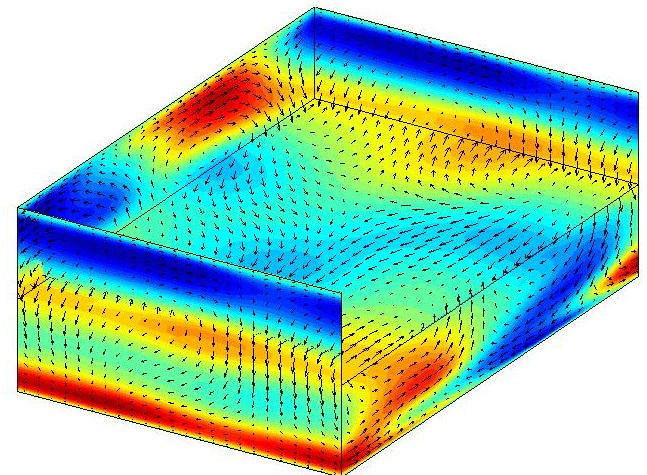
\includegraphics[scale=0.4]{Data/p8p32NoBase}}
\begin{itemize}
\item<1-> Even though it's in a reduced symmetry subspace that allows travelling waves, it has no relative velocity.
\end{itemize}
\end{frame}
\begin{frame}{P8.32}
\begin{itemize}
\item<1-> Coherent structures cannot exist for all Reynolds numbers - $Re = 0$ means only the laminar state can exist
\item <2-> Coherent structures will arise from some high-dimensional bifurcation 
\end{itemize}
\pause
\hspace{2cm} 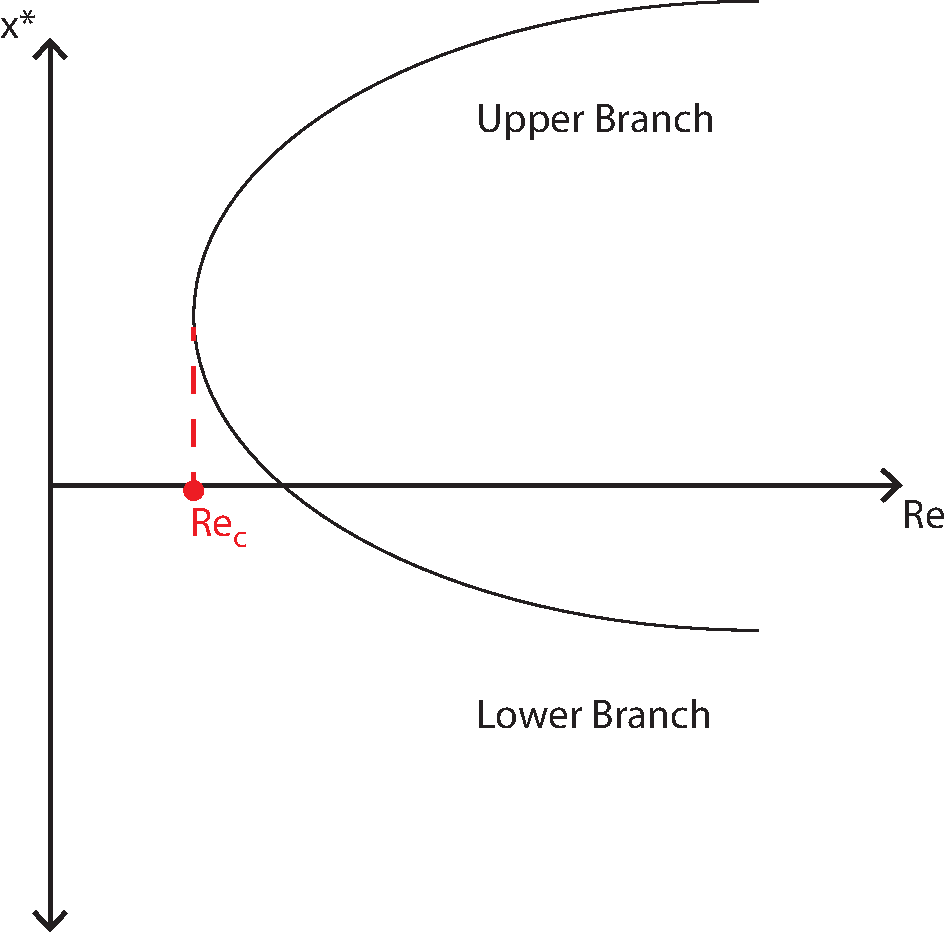
\includegraphics[scale=0.3]{Images/bifurcationDiagram.pdf}
\end{frame}

\begin{frame}{P8.32}
\begin{itemize}
\item <1-> Near bifurcation, period will be low - is P8.32 near a bifurcation? 
\item <2-> Can try to continue this solution for lower Reynolds numbers to locate the bifurcation
\item <3-> After bifurcation, coherent structures tend to branch off in pairs - can this orbit's pair be located?
\end{itemize}
\end{frame}
\section{Future Work} 
\begin{frame}{Future Work}
\begin{itemize}
\item<1-> Try to find travelling coherent structures in the reduced symmetry space
\item<2-> Try to find coherent structures in spaces with even less symmetry than P8.32
\item<3-> Find the bifurcation for P8.32 and continue the solution to find the other branch 
\end{itemize}
\end{frame}

{\aauwavesbg%
\begin{frame}[plain,noframenumbering]%
  \finalpage{Acknowledgments:
\begin{itemize}
\item<1-> John Gibson at UNH for making the subject approachable
\item<1-> Daniel Borrero for being a great thesis advisor 
\end{itemize}}
\end{frame}}
%%%%%%%%%%%%%%%%

\end{document}
